% Contenido de la sesión de 180 minutos (con una pausa de 10).
% Cada slide lleva una etiqueta (label) que el guion docente usa para sincronizarse.
% Las notas \note{...} quedan ocultas al proyectar.

% S01
{
  \setbeamertemplate{navigation symbols}{}
  \setbeamertemplate{footline}{}
  \begin{frame}[plain,label=portada]
    \titlepage
  \end{frame}
}

% ============================================================================
%  1. MOTIVACIÓN  (0--20 min)
% ============================================================================
\section{Motivación}

% S02
\begin{frame}[label=pregunta]{La productividad sube 0.72\% por un trimestre}
  \textbf{¿Qué hace la economía?}\par
  \vspace{0.45cm}
  ¿Trabajan más o menos los hogares?\par
  \vspace{0.15cm}
  ¿Consumen la ganancia o la ahorran?\par
  \vspace{0.15cm}
  ¿Cuánto dura el efecto?\par
  \vspace{0.6cm}
  Al final de la sesión, cada respuesta será un número, y cada número saldrá de una
  ecuación que ya conocen y de un archivo que habrán escrito ustedes.
  \note{Pedir predicciones a mano alzada: ¿las horas suben o bajan? Anotar la votación
  en la pizarra y volver a ella en el Acto 1 (slide acto1-horas). El 0.72\% es una
  desviación estándar del choque de PTF en la calibración de King y Rebelo (1999).}
\end{frame}

% S03
\begin{frame}[label=pizarra]{Hasta dónde llega la pizarra}
  \begin{columns}[T,onlytextwidth]
    \begin{column}{0.47\textwidth}
      \textbf{Depreciación total, $\delta=1$}\par
      \vspace{0.25cm}
      Solución cerrada (PD06, parte E).\par
      \vspace{0.2cm}
      $\hat h_t=0$: las horas no se mueven.\par
      \vspace{0.2cm}
      $\hat c_t=\hat y_t$: el hogar consume siempre la misma fracción.
    \end{column}
    \begin{column}{0.47\textwidth}
      \textbf{Caso realista, $\delta=0.025$}\par
      \vspace{0.25cm}
      No hay solución cerrada (PD06, E.3).\par
      \vspace{0.2cm}
      Las horas \emph{sí} responden.\par
      \vspace{0.2cm}
      Hay que resolver numéricamente.
    \end{column}
  \end{columns}
  \vspace{0.6cm}
  \begin{block}{La paradoja}
    El mecanismo que hace interesante al RBC aparece justo donde la pizarra deja de
    alcanzar.
  \end{block}
  \note{Conectar con la recitación: los alumnos ya probaron en E.3 que con $\delta<1$ el
  supuesto $\hat h_t=0$ es incompatible con la Euler. La sesión de hoy es la parte G:
  ``beyond the blackboard''.}
\end{frame}

% S04
\begin{frame}[label=laboratorio]{El modelo como laboratorio}
  \begin{quote}
    \enquote{Our task, as I see it \ldots\ is to write a FORTRAN program that will accept
    specific economic policy rules as `input' and will generate as `output' statistics
    describing the operating characteristics of time series we care about.}
  \end{quote}
  \begin{flushright}\small\parencite[pp.~709--710]{lucas1980}\end{flushright}
  \vspace{0.1cm}
  \begin{quote}
    \enquote{The key tool macroeconomists use is the computational experiment.}
  \end{quote}
  \begin{flushright}\small\parencite[p.~341]{kydland2004}\end{flushright}
  \vspace{0.1cm}

  En 1980 el programa de investigación ya se pensaba como código.
  \note{Subrayar la fecha. Kydland y Prescott (1982) convirtieron la visión de Lucas en
  método: calibrar el modelo como un instrumento de medición y luego interrogarlo.}
\end{frame}

% S05
\begin{frame}[label=linea-tiempo]{De la visión a la herramienta}
  \centering
  \begin{tikzpicture}[font=\footnotesize]
    \draw[very thick, upblue] (0,0) -- (9.8,0);
    \foreach \x/\y/\a in {
        0.6/1976/{Crítica\\de Lucas},
        2.3/1980/{Lucas,\\Blanchard--\\Kahn},
        4.0/1982/{Kydland--\\Prescott},
        5.7/1983/{Fair--Taylor},
        7.4/1994/{Juillard crea\\\textbf{Dynare}},
        9.1/2025/{30 años}}{
      \filldraw[upblue] (\x,0) circle (2.4pt);
      \node[upblue, font=\footnotesize\bfseries] at (\x,0.38) {\y};
      \node[align=center, text width=1.6cm, font=\scriptsize] at (\x,-0.8) {\a};
    }
  \end{tikzpicture}
  \par\vspace{0.6cm}
  \raggedright
  \textbf{Blanchard y Kahn (1980)}: cuándo un modelo lineal tiene solución única y
  estable. Es lo que Dynare comprueba con \cod{check}.\par
  \vspace{0.25cm}
  \textbf{Fair y Taylor (1983)}: el método para modelos no lineales de previsión
  perfecta.\par
  \vspace{0.25cm}
  \textbf{Dynare (1994, CEPREMAP)}: Michel Juillard une todo en un solo programa.
  \fuente{\parencite{bk1980,ft1983,kp1982,dynare}}
  \note{Cinco minutos como máximo. En febrero de 2025 el Banque de France celebró los
  treinta años de Dynare con una conferencia.}
\end{frame}

% S06
\begin{frame}[label=que-es-dynare]{¿Qué es Dynare?}
  \begin{bluebox}{Dynare}
    Un \textbf{preprocesador} y una biblioteca de rutinas para MATLAB u Octave que
    resuelve, simula y estima modelos DSGE.
  \end{bluebox}
  \vspace{0.2cm}
  Escribimos el modelo casi como en el papel. Dynare se encarga de:
  \begin{itemize}
    \item Estado estacionario y su verificación.
    \item Linealización con derivadas exactas.
    \item Condición de Blanchard--Kahn y regla de decisión.
    \item Funciones de impulso-respuesta y momentos.
    \item Estimación bayesiana (solo un adelanto al final).
  \end{itemize}
  \fuente{\parencite{dynare}}
  \note{Mencionar alternativas (Python, Julia) y por qué usamos Dynare: sintaxis
  declarativa, estándar en bancos centrales y licencia de MATLAB en la UP.}
\end{frame}

% S07
\begin{frame}[label=objetivos]{Al terminar la sesión}
  \begin{enumerate}
    \item Escribirás un \texttt{.mod} completo del modelo RBC.\par\vspace{0.15cm}
    \item Leerás lo que imprime Dynare: estado estacionario, valores propios y regla de
      decisión.\par\vspace{0.15cm}
    \item Explicarás cada impulso-respuesta con una ecuación.\par\vspace{0.15cm}
    \item Confrontarás el modelo con los datos.
  \end{enumerate}
  \vspace{0.4cm}
  \textbf{Material}\par
  \vspace{0.1cm}
  Handout \emph{Un crash course de Dynare}\par
  Taller \texttt{rbc\_taller.mod}\par
  PD06, parte G
  \note{Comprobar que todos tienen MATLAB abierto y la carpeta del taller descargada.
  Si alguien no tiene Dynare instalado, que trabaje en pareja.}
\end{frame}

% ============================================================================
%  2. EL MODELO  (20--50 min)
% ============================================================================
\section{Modelo}

% S08
\begin{frame}[label=impulso]{Impulso y propagación}
  \centering
  \begin{tikzpicture}[
    bx/.style={draw=darkblue, thick, rounded corners=3pt, fill=thmblue, align=center,
      text width=2.55cm, minimum height=1.35cm, font=\small},
    go/.style={-{Stealth[length=2.2mm]}, very thick, darkblue}]
    \node[bx] (a) at (0,0) {\textbf{Impulso}\\[2pt]\footnotesize choque de PTF, $\varepsilon_t$};
    \node[bx] (b) at (3.65,0) {\textbf{Propagación}\\[2pt]\footnotesize capital y decisiones del hogar};
    \node[bx] (c) at (7.3,0) {\textbf{Fluctuaciones}\\[2pt]\footnotesize $y,c,i,h$ persistentes};
    \draw[go] (a) -- (b); \draw[go] (b) -- (c);
  \end{tikzpicture}
  \par\vspace{0.6cm}\raggedright
  Un choque que dura \textbf{un trimestre} genera respuestas que duran
  \textbf{años}.\par
  \vspace{0.3cm}
  ¿De dónde sale esa persistencia? Dos candidatos:\par
  \vspace{0.15cm}
  \hspace*{0.4cm}la propia persistencia del choque, $\phi=0.979$;\par
  \hspace*{0.4cm}la acumulación de capital.\par
  \vspace{0.3cm}
  Al final veremos cuál de los dos hace casi todo el trabajo.
  \note{La distinción impulso--propagación es de Frisch (1933). La respuesta (slide
  limites) es incómoda para el RBC: casi toda la persistencia viene del choque.}
\end{frame}

% S09
\begin{frame}[label=mercados]{Dos agentes, tres mercados}
  \centering
  \resizebox{\textwidth}{!}{%
  \begin{tikzpicture}[
    ag/.style={draw=darkblue, very thick, rounded corners=4pt, fill=thmblue, align=center,
      text width=2.4cm, minimum height=5.3cm, font=\small},
    mk/.style={draw=upblue, thick, rounded corners=2pt, fill=white, align=center,
      text width=2.3cm, minimum height=1.1cm, font=\small},
    fl/.style={-{Stealth[length=2mm]}, thick, darkblue},
    lab/.style={font=\footnotesize, align=center, text width=3cm, inner sep=1.5pt}]
    \node[ag] (H) at (0,0) {\textbf{HOGAR}\\[6pt]\footnotesize elige $c_t$, $h_t$, $i_t$\\[4pt]
      \footnotesize posee el capital};
    \node[ag] (F) at (11,0) {\textbf{FIRMA}\\[6pt]\footnotesize elige $h_t$, $k_{t-1}$\\[4pt]
      \footnotesize maximiza beneficios};
    \node[mk] (L) at (5.5,1.9) {\textbf{Trabajo}\\ $h_t$, $w_t$};
    \node[mk] (K) at (5.5,0) {\textbf{Capital}\\ $k_{t-1}$, $r_t$};
    \node[mk] (B) at (5.5,-1.9) {\textbf{Bienes}\\ $y_t$, precio 1};
    \draw[fl] (H.east|-L) -- node[lab, above]{oferta} node[lab, below]{$\theta\frac{c_t}{1-h_t}=w_t$} (L.west);
    \draw[fl] (F.west|-L) -- node[lab, above]{demanda} node[lab, below]{$w_t=\alpha\frac{y_t}{h_t}$} (L.east);
    \draw[fl] (H.east|-K) -- node[lab, above]{oferta: elegida} node[lab, below]{ayer, con la Euler} (K.west);
    \draw[fl] (F.west|-K) -- node[lab, above]{demanda} node[lab, below]{$r_t=(1-\alpha)\frac{y_t}{k_{t-1}}$} (K.east);
    \draw[fl] (H.east|-B) -- node[lab, above]{demanda} node[lab, below]{$c_t+i_t$} (B.west);
    \draw[fl] (F.west|-B) -- node[lab, above]{oferta} node[lab, below]{$y_t$} (B.east);
    \node[font=\footnotesize, text=errframe, align=center] (S) at (11,3.6) {choque: $\ln a_t=\phi\ln a_{t-1}+\varepsilon_t$};
    \draw[-{Stealth[length=2mm]}, thick, errframe] (S.south) -- (F.north);
  \end{tikzpicture}}
  \par\vspace{0.3cm}\raggedright
  Cada flecha es una ecuación. El choque entra por la firma; el hogar lo siente a
  través de los precios $w_t$ y $r_t$.
  \fuente{Notación de Dynare: $k_{t-1}$ es el capital que se usa en $t$. Inspirada en
  \textcite[Fig.~3.1]{gmo}.}
  \note{Usar esta lámina como mapa: en el Acto 1 volveremos a ella mercado por mercado.}
\end{frame}

% S10
\begin{frame}[label=hogar]{El hogar}
  \begin{gather*}
  \max_{\{c_t,h_t,k_t\}}\ \mathbb{E}_0\sum_{t=0}^{\infty}\beta^t\big[\ln c_t+\theta\ln(1-h_t)\big]\\
  \text{s.a.}\quad c_t+k_t=w_th_t+(r_t+1-\delta)\,k_{t-1}
  \end{gather*}
  \par\vspace{0.2cm}
  \textbf{Euler} (ahorrar hoy, consumir mañana)
  \[
  \frac{1}{c_t}=\beta\,\mathbb{E}_t\!\left[\frac{1}{c_{t+1}}\,(r_{t+1}+1-\delta)\right]
  \]
  \textbf{Oferta de trabajo} (ocio contra consumo)
  \[
  \theta\,\frac{c_t}{1-h_t}=w_t
  \]
  \par\vspace{0.1cm}
  ¿Qué retorno decide el ahorro de hoy: el de hoy o el de mañana?
  \note{La pregunta prepara el hueco H8: en Dynare, \texttt{r(+1)} y \texttt{c(+1)}.
  La restricción usa $k_t=(1-\delta)k_{t-1}+i_t$ ya sustituida.}
\end{frame}

% S11
\begin{frame}[label=firma]{La firma y el choque}
  \[
  \max_{h_t,\,k_{t-1}}\ y_t-w_th_t-r_tk_{t-1},\qquad y_t=a_t\,k_{t-1}^{1-\alpha}h_t^{\alpha}
  \]
  \par\vspace{0.15cm}
  \textbf{Demandas de factores}
  \[
  w_t=\alpha\,\frac{y_t}{h_t},\qquad r_t=(1-\alpha)\,\frac{y_t}{k_{t-1}}
  \]
  \textbf{Productividad}
  \[
  \ln a_t=\phi\ln a_{t-1}+\sigma_\varepsilon\,\varepsilon_t,\qquad \varepsilon_t\sim N(0,1)
  \]
  \par\vspace{0.1cm}
  Atención: aquí $\alpha$ es la participación del \textbf{trabajo}, no la del capital.
  \note{King y Rebelo (1999) usan esta convención. Es una fuente frecuente de errores al
  copiar fórmulas de otros textos.}
\end{frame}

% S12
\begin{frame}[label=equilibrio]{Ocho ecuaciones, ocho incógnitas}
  \centering\small
  \renewcommand{\arraystretch}{1.35}
  \begin{tabular}{@{}lll@{}}
    \toprule
    & \textbf{Ecuación} & \\
    \midrule
    1 & $1/c_t=\beta\,\mathbb{E}_t[(r_{t+1}+1-\delta)/c_{t+1}]$ & Euler\\
    2 & $\theta\,c_t/(1-h_t)=w_t$ & oferta de trabajo\\
    3 & $r_t=(1-\alpha)\,y_t/k_{t-1}$ & demanda de capital\\
    4 & $w_t=\alpha\,y_t/h_t$ & demanda de trabajo\\
    5 & $y_t=a_t\,k_{t-1}^{1-\alpha}h_t^{\alpha}$ & producción\\
    6 & $k_t=(1-\delta)\,k_{t-1}+i_t$ & ley de movimiento\\
    7 & $y_t=c_t+i_t$ & vaciado de bienes\\
    8 & $\ln a_t=\phi\ln a_{t-1}+\sigma_\varepsilon\varepsilon_t$ & productividad\\
    \bottomrule
  \end{tabular}
  \par\vspace{0.35cm}\raggedright
  Incógnitas: $y_t,c_t,i_t,k_t,h_t,r_t,w_t,a_t$. Esta lista \emph{es} el bloque
  \cod{model} de Dynare.
  \note{Lo primero que hace Dynare es contar: ecuaciones = variables endógenas.}
\end{frame}

% S13
\begin{frame}[label=ee]{El estado estacionario, en cascada}
  Sin choques y sin tiempo. Cada paso usa solo lo anterior:
  \vspace{0.15cm}
  \begin{align*}
    r_{ss}&=\tfrac{1}{\beta}-(1-\delta) &&= 0.0413 \\
    k_{ss}&=h_{ss}\big[(1-\alpha)/r_{ss}\big]^{1/\alpha} &&= 4.5785\\
    y_{ss}&=k_{ss}^{1-\alpha}h_{ss}^{\alpha} &&= 0.5673\\
    i_{ss}&=\delta\,k_{ss},\qquad c_{ss}=y_{ss}-i_{ss} &&= 0.1145,\ 0.4528\\
    w_{ss}&=\alpha\,y_{ss}/h_{ss} &&= 1.8919\\
    \theta&=w_{ss}(1-h_{ss})/c_{ss} &&= \num{3.3424}
  \end{align*}
  \par\vspace{0.1cm}
  $\theta$ no se elige: se \textbf{calibra} para que las horas de estado estacionario
  sean $h_{ss}=0.20$.
  \note{Son los huecos H3 a H7 del taller. El orden importa: $\theta$ va al final porque
  los niveles de estado estacionario no dependen de él.}
\end{frame}

% S14
\begin{frame}[label=calibracion]{Calibración trimestral}
  \centering\small
  \renewcommand{\arraystretch}{1.15}
  \begin{tabular}{@{}llr@{}}
    \toprule
    \textbf{Parámetro} & \textbf{Significado} & \textbf{Valor}\\
    \midrule
    $\alpha$ & participación del trabajo & $0.667$\\
    $\beta$ & factor de descuento & $0.984$\\
    $\delta$ & depreciación & $0.025$\\
    $\phi$ & persistencia de la PTF & $0.979$\\
    $\sigma_\varepsilon$ & desviación estándar del choque & $0.0072$\\
    $h_{ss}$ & horas de estado estacionario (objetivo) & $0.20$\\
    \midrule
    $\theta$ & peso del ocio (calibrado) & $3.3424$\\
    \bottomrule
  \end{tabular}
  \fuente{\textcite{kingrebelo1999}.}
  \par\vspace{0.2cm}\raggedright\normalsize
  Calibrar: fijar los parámetros con información de largo plazo y luego preguntarle al
  modelo lo que no sabemos.
  \note{Recordar la frase de Kydland: los modelos son instrumentos de medición que hay
  que calibrar.}
\end{frame}

% S15
\begin{frame}[label=loglineal]{El sistema log-lineal}
  Con $\hat x_t=\ln(x_t/x_{ss})$, en desviaciones porcentuales:
  \small
  \begin{align*}
    \hat y_t&=\hat a_t+(1-\alpha)\hat k_t+\alpha\hat h_t &
    \hat r_t&=\hat y_t-\hat k_t\\
    \hat w_t&=\hat y_t-\hat h_t &
    \hat c_t+\tfrac{h_{ss}}{1-h_{ss}}\hat h_t&=\hat w_t\\
    \mathbb{E}_t\hat c_{t+1}-\hat c_t&=\beta r_{ss}\,\mathbb{E}_t\hat r_{t+1} &
    \hat k_{t+1}&=(1-\delta)\hat k_t+\delta\hat\imath_t\\
    \hat y_t&=s_c\hat c_t+s_i\hat\imath_t &
    \hat a_t&=\phi\hat a_{t-1}+\varepsilon_t
  \end{align*}
  \normalsize
  \vspace{0.1cm}
  Notación de la pizarra: $\hat k_t$ es el capital en uso en $t$.\par
  \vspace{0.2cm}
  $s_c=0.798$, $s_i=0.202$, $\beta r_{ss}=0.0406$, $\tfrac{h_{ss}}{1-h_{ss}}=0.25$.\par
  \vspace{0.25cm}
  Dynare hará esta linealización por nosotros, con derivadas exactas.
  \note{No es necesario escribir este sistema en Dynare. Lo usaremos para leer las IRF en
  la sección de resultados.}
\end{frame}

% S16
\begin{frame}[label=bk]{Blanchard--Kahn en una lámina}
  Reducido a $(\hat k_t,\hat a_t,\hat c_t)$, el sistema tiene tres valores propios:
  \vspace{0.25cm}
  \begin{center}
    \renewcommand{\arraystretch}{1.3}
    \begin{tabular}{@{}lccc@{}}
      \toprule
      Valor propio & $0.936$ & $0.979=\phi$ & $1.086$\\
      ¿Estable? & sí & sí & \textbf{no}\\
      \bottomrule
    \end{tabular}
  \end{center}
  \vspace{0.2cm}
  Una raíz inestable para una variable que salta ($\hat c_t$): \textbf{solución única}.\par
  \vspace{0.3cm}
  El consumo elige, en cada trimestre, el único valor que no lleva a una trayectoria
  explosiva: el \textbf{brazo estable del punto de silla}.\par
  \vspace{0.3cm}
  Dynare verificará esto con el comando \cod{check}.
  \fuente{\textcite{bk1980}; PD06, partes F.3 y F.4.}
  \note{Si sobran raíces inestables, no hay solución acotada; si faltan, hay infinitas
  (indeterminación). Ambos mensajes los veremos en Dynare.}
\end{frame}

% S17
\begin{frame}[label=reparto]{Quién hace qué}
  \centering
  \renewcommand{\arraystretch}{1.35}
  \begin{tabular}{@{}lcc@{}}
    \toprule
    \textbf{Paso} & \textbf{Tú} & \textbf{Dynare}\\
    \midrule
    Condiciones de primer orden & \faCheck & \\
    Estado estacionario cerrado & \faCheck & lo verifica\\
    Calibración & \faCheck & \\
    Linealización & & \faCheck\\
    Blanchard--Kahn & & \faCheck\\
    Regla de decisión & & \faCheck\\
    IRF y momentos & & \faCheck\\
    \textbf{Interpretación} & \faCheck & \\
    \bottomrule
  \end{tabular}
  \par\vspace{0.4cm}\raggedright
  La economía la pones tú, al principio y al final. Dynare hace el álgebra del medio.
  \note{Transición a la parte práctica. Abrir MATLAB.}
\end{frame}

% ============================================================================
%  3. DYNARE EN VIVO  (50--115 min)
% ============================================================================
\section{Dynare}

% S18
\begin{frame}[label=preprocesador]{Dynare traduce, MATLAB ejecuta}
  \centering
  \resizebox{\textwidth}{!}{%
  \begin{tikzpicture}[
    doc/.style={draw=darkblue, thick, fill=white, minimum width=1.7cm, minimum height=2.1cm,
      align=center, font=\small},
    fil/.style={draw=errframe!70, fill=errframe!8, rounded corners=1pt, font=\ttfamily\small,
      text width=3.5cm, inner sep=2.5pt, align=center},
    res/.style={draw=darkblue, fill=thmblue, rounded corners=2pt, font=\ttfamily\small,
      minimum width=1.7cm, inner sep=3pt},
    go/.style={-{Stealth[length=2.3mm]}, very thick, darkblue}]
    \node[doc] (mod) at (-0.6,0) {\ttfamily rbc\_\\\ttfamily taller\\\ttfamily .mod};
    \node[fil] (f1) at (4.6,0.9) {driver.m};
    \node[fil] (f2) at (4.6,0.3) {static\_resid.m, \ldots};
    \node[fil] (f3) at (4.6,-0.3) {dynamic\_g1.m, \ldots};
    \node[fil] (f4) at (4.6,-0.9) {steadystate.m};
    \node[res] (M) at (8.6,0.8) {M\_};
    \node[res] (op) at (8.6,0) {options\_};
    \node[res] (oo) at (8.6,-0.8) {oo\_};
    \begin{scope}[on background layer]
      \node[draw=darkblue, very thick, rounded corners=6pt, fill=thmblue!35,
        fit=(f1)(f4)(M)(oo), inner xsep=9pt, inner ysep=11pt] (mat) {};
    \end{scope}
    \node[font=\bfseries\small, text=darkblue, anchor=south] at (mat.north) {MATLAB};
    \draw[go] (mod.east) -- node[above=2pt, font=\footnotesize, align=center]{pre-\\procesador} (mod.east -| mat.west);
    \draw[go] ($(f2.east)!0.5!(f3.east)+(0.1,0)$) -- ($(op.west)+(-0.1,0)$);
    \node[font=\footnotesize\itshape, text=darkblue] at (-0.6,-1.6) {lo que escribes};
    \node[font=\footnotesize\itshape, text=darkblue] at (4.6,-1.8) {lo que genera Dynare};
    \node[font=\footnotesize\itshape, text=darkblue] at (8.6,-1.8) {resultados};
  \end{tikzpicture}}
  \par\vspace{0.5cm}\raggedright
  \texttt{dynare rbc\_taller} lee el \texttt{.mod}, comprueba la sintaxis, calcula las
  derivadas \textbf{analíticamente} y escribe archivos de MATLAB.\par
  \vspace{0.25cm}
  Los resultados quedan en tres estructuras: \cod{M\_} (el modelo), \cod{options\_}
  (las opciones) y \cod{oo\_} (los resultados).
  \fuente{Inspirada en \textcite[Fig.~2.1]{gmo}.}
\end{frame}

% S19
\begin{frame}[fragile,label=arranque]{Antes de escribir una línea}
  \begin{lstlisting}[language={}]
>> addpath C:\dynare\7.1\matlab     % una vez por sesion
>> cd <carpeta del taller>
>> edit rbc_taller.mod              % abre el archivo
\end{lstlisting}
  \vspace{0.3cm}
  El archivo tiene \textbf{20 huecos} \texttt{???}, numerados \texttt{[H1]} a
  \texttt{[H20]}, ordenados según los cinco bloques de un \texttt{.mod}.\par
  \vspace{0.3cm}
  Cada hueco trae una pista y la sección del handout que lo explica.\par
  \vspace{0.3cm}
  Dynare no corre mientras quede un \texttt{???} activo. Si lo intentas:
  \begin{lstlisting}[language={}]
ERROR: rbc_taller.mod: line 37, col 5: character
       unrecognized by lexer
\end{lstlisting}
  \note{Que todos corran el archivo sin tocarlo y vean este error: así lo reconocen
  después. La línea 37 es el hueco H1.}
\end{frame}

% S20
\begin{frame}[label=bloques]{Los cinco bloques de un \texttt{.mod}}
  \centering
  \renewcommand{\arraystretch}{1.45}
  \begin{tabular}{@{}cl>{\raggedright\arraybackslash}p{4.4cm}c@{}}
    \toprule
    & \textbf{Bloque} & \textbf{Qué contiene} & \textbf{Huecos}\\
    \midrule
    1 & Preámbulo & \texttt{var}, \texttt{varexo}, \texttt{parameters} y calibración & H1--H7\\
    2 & Modelo & las ocho ecuaciones & H8--H15\\
    3 & Estado estacionario & \texttt{steady\_state\_model} & H16--H17\\
    4 & Choques & \texttt{shocks} & H18\\
    5 & Cálculo & \texttt{steady}, \texttt{check}, \texttt{stoch\_simul} & H19--H20\\
    \bottomrule
  \end{tabular}
  \par\vspace{0.4cm}\raggedright
  El orden no es arbitrario: es el orden en que Dynare necesita la información.
  \fuente{Handout, §3.2. Inspirada en \textcite[Fig.~2.2]{gmo}.}
\end{frame}

% S21
\begin{frame}[fragile,label=etapa1]{Etapa 1: el preámbulo}
  \begin{lstlisting}
var y c i k h r w a;      // [H1] 8 endogenas
varexo eps;               // [H2] el choque
parameters alpha beta delta phi sigma_eps theta hss
           r_ss k_ss y_ss i_ss c_ss w_ss;
alpha = 0.667;            // ... calibracion
r_ss  = ???;              // [H3]  (lamina ee)
k_ss  = ???;              // [H4]
theta = ???;              // [H7]
\end{lstlisting}
  \vspace{0.2cm}
  Un parámetro puede definirse a partir de otros ya asignados: así calculamos el estado
  estacionario cerrado sin resolver nada.\par
  \vspace{0.25cm}
  \textbf{10 minutos.} Completa H1--H7 con la lámina del estado estacionario.
  \note{Respuestas en el solucionario. Error típico en H4: usar $\alpha$ como
  participación del capital.}
\end{frame}

% S22
\begin{frame}[label=reglas]{Etapa 2: cómo se escribe una ecuación}
  \begin{enumerate}
    \item Una ecuación por línea, terminada en \texttt{;}.\par\vspace{0.12cm}
    \item El tiempo va entre paréntesis: \texttt{c(+1)} es $c_{t+1}$ y \texttt{k(-1)} es
      $k_{t-1}$.\par\vspace{0.12cm}
    \item No se escribe $\mathbb{E}_t$: todo \texttt{(+1)} está en esperanza.\par\vspace{0.12cm}
    \item Operaciones como en MATLAB: \texttt{*}, \texttt{/}, \texttt{\^{}},
      \texttt{log()}, \texttt{exp()}.\par\vspace{0.12cm}
    \item Una etiqueta \texttt{[name='Euler']} antes de la ecuación ayuda a leer los
      errores.
  \end{enumerate}
  \vspace{0.3cm}
  \begin{block}{La regla que más errores evita}
    Cada variable se fecha por el período en que \textbf{se decide}.
  \end{block}
\end{frame}

% S23
\begin{frame}[label=timing]{El timing del capital}
  \centering
  \begin{tikzpicture}[font=\small, >={Stealth[length=2mm]}]
    \draw[thick, ->] (0,0) -- (10,0) node[right]{$t$};
    \foreach \x/\l in {1.5/{$t-1$}, 5/{$t$}, 8.5/{$t+1$}}{
      \draw[thick] (\x,0.12) -- (\x,-0.12) node[below]{\l};}
    \draw[very thick, darkblue, ->] (1.6,0.35) to[bend left=30]
      node[above, align=center]{se elige en $t-1$,\\ se usa en $t$} (4.9,0.35);
    \node[draw=darkblue, fill=thmblue, rounded corners=2pt, align=center] at (3.25,-1.35)
      {Pizarra: $k_t$\\ Dynare: \texttt{k(-1)}};
    \draw[very thick, errframe, ->] (5.1,0.35) to[bend left=30]
      node[above, align=center]{se elige en $t$,\\ se usa en $t+1$} (8.4,0.35);
    \node[draw=errframe, fill=errframe!8, rounded corners=2pt, align=center] at (6.75,-1.35)
      {Pizarra: $k_{t+1}$\\ Dynare: \texttt{k}};
  \end{tikzpicture}
  \par\vspace{0.4cm}\raggedright
  En Dynare, \texttt{k} es el capital elegido \emph{hoy}. El que produce hoy es
  \texttt{k(-1)}.\par
  \vspace{0.2cm}
  Producción y demanda de capital deben usar \texttt{k(-1)}; la ley de movimiento
  escribe \texttt{k} a la izquierda.
  \fuente{Handout, §3.2.2.}
  \note{Es el error número uno. Preguntar: en la ley de movimiento, ¿qué capital va a la
  izquierda?}
\end{frame}

% S24
\begin{frame}[label=etapa2]{Etapa 2: del papel al código}
  \centering\small
  \renewcommand{\arraystretch}{1.4}
  \begin{tabular}{@{}cll@{}}
    \toprule
    \textbf{Hueco} & \textbf{Papel} & \textbf{Pista}\\
    \midrule
    H8 & $1/c_t=\beta\,\mathbb{E}_t[(r_{t+1}+1-\delta)/c_{t+1}]$ & retorno de mañana\\
    H9 & $\theta c_t/(1-h_t)=w_t$ & \\
    H10 & $r_t=(1-\alpha)y_t/k_{t-1}$ & timing\\
    H11 & $w_t=\alpha y_t/h_t$ & \\
    H12 & $y_t=a_tk_{t-1}^{1-\alpha}h_t^{\alpha}$ & timing\\
    H13 & $k_t=(1-\delta)k_{t-1}+i_t$ & \\
    H14 & $y_t=c_t+i_t$ & \\
    H15 & $\ln a_t=\phi\ln a_{t-1}+\sigma_\varepsilon\varepsilon_t$ & en logaritmos\\
    \bottomrule
  \end{tabular}
  \par\vspace{0.35cm}\raggedright
  \textbf{15 minutos.} Escribe las ocho ecuaciones en el bloque \texttt{model}.
  \note{Caminar por el aula. Revisar H8 (r(+1)), H10 y H12 (k(-1)) en cada pantalla.}
\end{frame}

% S25
\begin{frame}[fragile,label=etapa2-sol]{Etapa 2 resuelta}
  \begin{lstlisting}
model;
  1/c = beta*(1/c(+1))*(r(+1) + 1 - delta);   // H8
  theta*c/(1 - h) = w;                        // H9
  r = (1 - alpha)*y/k(-1);                    // H10
  w = alpha*y/h;                              // H11
  y = a*k(-1)^(1 - alpha)*h^alpha;            // H12
  k = (1 - delta)*k(-1) + i;                  // H13
  y = c + i;                                  // H14
  log(a) = phi*log(a(-1)) + sigma_eps*eps;    // H15
end;
\end{lstlisting}
  \vspace{0.2cm}
  Ocho ecuaciones, casi idénticas a la pizarra. La única traducción real es el
  \textbf{timing}.
  \note{Mostrar solo después de que la mayoría haya intentado. Las etiquetas
  [name=...] se omiten aquí por espacio; en el archivo están.}
\end{frame}

% S26
\begin{frame}[fragile,label=etapa34]{Etapas 3 y 4: estado estacionario y choque}
  \begin{lstlisting}
steady_state_model;
  a = ???;               // [H16]  ojo: a, no ln a
  r = r_ss;  h = hss;
  k = ???;  y = ???;  i = ???;  c = ???;  w = ???;  // [H17]
end;

shocks;
  var eps; stderr ???;   // [H18]
end;
\end{lstlisting}
  \vspace{0.2cm}
  \texttt{steady\_state\_model} no resuelve nada: solo \textbf{evalúa} las fórmulas
  cerradas del preámbulo.\par
  \vspace{0.25cm}
  ¿Por qué \texttt{stderr} no debería ser $0.0072$?
  \note{H16 = 1 (ln 1 = 0; con 0, log(0) no existe). H18 = 1: sigma\_eps ya escala el
  choque dentro de la PTF; con 0.0072 el choque queda escalado dos veces y las IRF salen
  139 veces más chicas.}
\end{frame}

% S27
\begin{frame}[fragile,label=control1]{Punto de control 1: \texttt{steady} y \texttt{resid}}
  \begin{lstlisting}[language={}]
>> dynare rbc_taller
\end{lstlisting}
  \vspace{0.1cm}
  \centering\small
  \texttt{STEADY-STATE RESULTS}\par\vspace{0.1cm}
  \begin{tabular}{@{}cccccccc@{}}
    \toprule
    $y$ & $c$ & $i$ & $k$ & $h$ & $r$ & $w$ & $a$\\
    \midrule
    0.5673 & 0.4528 & 0.1145 & 4.5785 & 0.2000 & 0.0413 & 1.8919 & 1.0000\\
    \bottomrule
  \end{tabular}
  \par\vspace{0.35cm}\raggedright\normalsize
  Los ocho residuos deben salir en \texttt{0.000000}.\par
  \vspace{0.2cm}
  Escribe \texttt{theta} en la ventana de comandos: \num{3.3424}.\par
  \vspace{0.3cm}
  \begin{block}{Si un residuo no es cero}
    Hay un error de álgebra en el estado estacionario. La ecuación con residuo es la
    sospechosa.
  \end{block}
  \note{Un residuo cero no garantiza que el modelo esté bien: si en H13 alguien escribió
  k = (1-delta)*k + i, el estado estacionario cuadra igual. Lo delata el control 3.}
\end{frame}

% S28
\begin{frame}[fragile,label=control2]{Punto de control 2: \texttt{check} (H19)}
  \begin{lstlisting}[language={}]
EIGENVALUES:
   Modulus      Real   Imaginary
     0.936     0.936           0
     0.979     0.979           0
     1.086     1.086           0
 1.145e+18 1.145e+18           0
There are 2 eigenvalue(s) larger than 1 in modulus
for 2 forward-looking variable(s).
The order and rank conditions are verified.
\end{lstlisting}
  \vspace{0.15cm}
  $0.936$, $0.979$ y $1.086$: los de la pizarra.\par
  \vspace{0.15cm}
  ¿Y el gigante? \texttt{r} aparece como \texttt{r(+1)} en la Euler, así que Dynare la
  cuenta como variable que salta. Es estática: su valor propio es infinito. Dos raíces
  inestables para dos \emph{jumpers}.
  \note{La economía es la misma: un solo salto genuino, el consumo. Si sustituimos r en la
  Euler, el valor propio infinito desaparece.}
\end{frame}

% S29
\begin{frame}[label=control3]{Punto de control 3: la regla de decisión (H20)}
  \centering\small
  \texttt{stoch\_simul(order = 1, irf = 40) y c i k h r w a;}\par
  \vspace{0.25cm}
  \setlength{\tabcolsep}{4.5pt}
  \begin{tabular}{@{}lrrrrr@{}}
    \toprule
    & $y$ & $c$ & $i$ & $k$ & $h$\\
    \midrule
    Constante & 0.5673 & 0.4528 & 0.1145 & 4.5785 & 0.2000\\
    \texttt{k(-1)} & 0.0134 & 0.0524 & $-0.0390$ & \num{0.9360} & $-0.0147$\\
    \texttt{a(-1)} & 0.8205 & 0.2584 & 0.5621 & 0.5621 & 0.1401\\
    \texttt{eps} & 0.0060 & 0.0019 & 0.0041 & 0.0041 & 0.0010\\
    \bottomrule
  \end{tabular}
  \par\vspace{0.3cm}\raggedright\normalsize
  Está en \textbf{niveles}: cada número es una desviación del estado estacionario.\par
  \vspace{0.15cm}
  La diagonal lleva el valor propio estable: el capital de hoy hereda $0.936$ del de
  ayer.\par
  \vspace{0.15cm}
  En elasticidad: $0.0524\times k_{ss}/c_{ss}=0.0524\times4.5785/0.4528=\num{0.530}$.
  \note{La fila eps es la del impacto: el primer punto de cada IRF. Es la fila a(-1)
  multiplicada por sigma/phi.}
\end{frame}

% S30
\begin{frame}[label=errores]{Lo que va a fallar}
  \footnotesize
  \renewcommand{\arraystretch}{1.2}
  \begin{tabular}{@{}>{\raggedright\arraybackslash}p{4.6cm}>{\raggedright\arraybackslash}p{5.6cm}@{}}
    \toprule
    \textbf{Síntoma} & \textbf{Causa probable}\\
    \midrule
    \texttt{character unrecognized by lexer} & queda un \texttt{???}\\
    Símbolo no declarado & falta en \texttt{var} o \texttt{parameters}\\
    Residuo distinto de cero & error en el estado estacionario\\
    Residuos no finitos & \texttt{a = 0} en \texttt{steady\_state\_model}: $\ln 0$\\
    \texttt{Blanchard \& Kahn conditions are not satisfied} & timing: \texttt{k(+1)} o \texttt{k} donde va \texttt{k(-1)}\\
    IRF 139 veces más chicas & \texttt{stderr 0.0072}: choque escalado dos veces\\
    Términos de segundo orden & falta \texttt{order = 1}: el valor por defecto es 2\\
    \bottomrule
  \end{tabular}
  \fuente{Handout, §3.13, ``Depuración''.}
  \note{El comando que se detiene localiza la avería: steady, resid, check, stoch\_simul,
  en ese orden.}
\end{frame}

% S31
\begin{frame}[label=donde-guarda]{Dónde quedan los resultados}
  \small
  \cod{oo\_.steady\_state}: estado estacionario.\par
  \cod{oo\_.irfs.c\_eps}: IRF del consumo, en niveles.\par
  \cod{oo\_.dr.ghx}, \cod{oo\_.dr.ghu}: regla de decisión.\par
  \vspace{0.15cm}
  \centering
  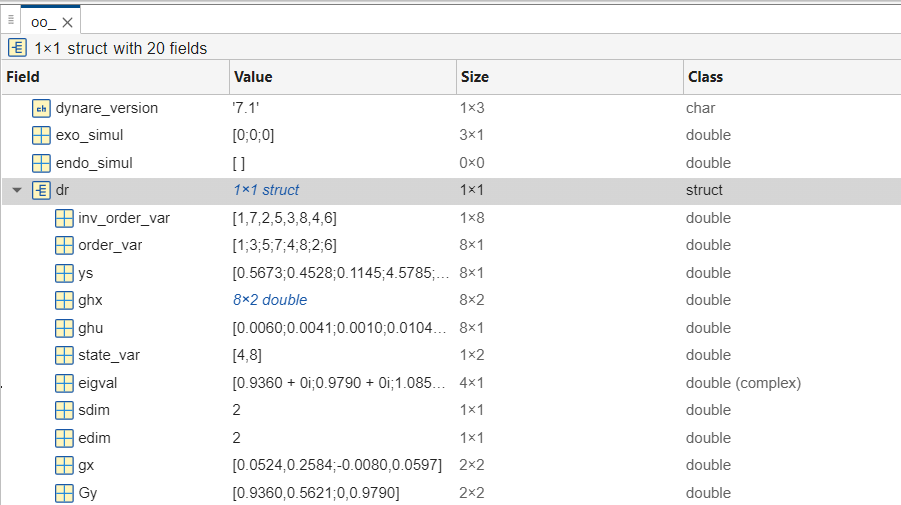
\includegraphics[width=0.72\textwidth]{04_oo_dr.png}\par
  \vspace{0.1cm}\raggedright
  \textbf{Trampa:} las filas de \texttt{ghx} siguen el \emph{orden DR}
  (\texttt{order\_var}), no el de \texttt{var}. La fila 2 es $i$, no $c$.\normalsize
  \fuente{Handout, §3.7. Captura de MATLAB con Dynare 7.1.}
  \note{\texttt{reconstruir\_irf.m} rearma las IRF desde ghx y ghu; coincide con
  oo\_.irfs hasta 4e-16.}
\end{frame}

% S32
{
\setbeamercolor{background canvas}{bg=UWBlack}
\begin{frame}[label=pausa]
  \centering\vfill
  {\color{UWGoldL3}\fontsize{28}{32}\selectfont\bfseries Pausa\par}
  \vspace{0.4cm}
  {\color{UWWhite}\large 10 minutos\par}
  \vspace{0.6cm}
  {\color{UWGrayL2}\small Al volver: ¿qué hace la economía con esos números?\par}
  \vfill
\end{frame}
}

% ============================================================================
%  4. RESULTADOS  (125--165 min)
%  Todas las cifras: regla de decisión de Dynare 7.1 (rbc_analytical.mod) en
%  elasticidades. Notación de la pizarra: \hat k_t es el capital en uso en t.
% ============================================================================
\section{Resultados}

% S33
\begin{frame}[label=receta]{La receta: de dónde sale cada número}
  \begin{columns}[T,onlytextwidth]
    \begin{column}{0.44\textwidth}
      \small
      \textbf{1. El choque}\par
      $\hat a_1=\sigma_\varepsilon=0.72\%$\par
      \vspace{0.25cm}
      \textbf{2. Condición inicial}\par
      $\hat k_1=0$: el capital ya estaba elegido.\par
      \vspace{0.25cm}
      \textbf{3. Los estados avanzan}\par
      $\hat a_{t+1}=0.979\,\hat a_t$\par
      $\hat k_{t+1}=0.936\,\hat k_t+0.125\,\hat a_t$\par
      \vspace{0.25cm}
      \textbf{4. Cada variable}\par
      $\hat x_t=\eta_{xk}\,\hat k_t+\eta_{xa}\,\hat a_t$
    \end{column}
    \begin{column}{0.52\textwidth}
      \centering\small
      \renewcommand{\arraystretch}{1.2}
      \begin{tabular}{@{}lrr@{}}
        \toprule
        & $\eta_{xk}$ & $\eta_{xa}$\\
        \midrule
        Producto $\hat y$ & 0.108 & 1.477\\
        Consumo $\hat c$ & 0.530 & 0.583\\
        Inversión $\hat\imath$ & $-1.560$ & 5.016\\
        Horas $\hat h$ & $-0.337$ & 0.716\\
        Salario $\hat w$ & 0.445 & 0.762\\
        Alquiler $\hat r$ & $-0.892$ & 1.477\\
        Capital $\hat k_{t+1}$ & 0.936 & 0.125\\
        \bottomrule
      \end{tabular}
    \end{column}
  \end{columns}
  \fuente{Regla de decisión de Dynare pasada a elasticidades, $\delta=0.025$.}
  \note{Las elasticidades salen del control 3: coeficiente en niveles por
  (estado)\_ss/x\_ss. Coinciden con las fórmulas de la PD06, F.5.}
\end{frame}

% S34
\begin{frame}[fragile,label=dynare-confirma]{Dynare da lo mismo, trimestre a trimestre}
  \begin{lstlisting}[language={}]
>> 100*oo_.irfs.y_eps(1:3)/oo_.steady_state(1)
    1.0636    1.0511    1.0381
>> 100*oo_.irfs.c_eps(1:3)/oo_.steady_state(2)
    0.4196    0.4586    0.4938
\end{lstlisting}
  \vspace{0.2cm}
  \texttt{oo\_.irfs} guarda 40 valores por variable, en niveles: se dividen por el
  estado estacionario para pasar a porcentaje.\par
  \vspace{0.25cm}
  El primer elemento es el trimestre del choque.\par
  \vspace{0.25cm}
  Cuidado: el \texttt{k} de Dynare es el capital \emph{elegido}. Su primer valor,
  $0.0903\%$, es el $\hat k_2$ de la pizarra.
  \note{Para la receta: y = 1.477 x 0.72 = 1.064; c = 0.583 x 0.72 = 0.420.}
\end{frame}

% S35
\begin{frame}[label=dos-ideas]{Dos ideas que ordenan la historia}
  \begin{columns}[T,onlytextwidth]
    \begin{column}{0.47\textwidth}
      \textbf{1. El choque es transitorio, aunque persistente}\par
      \vspace{0.25cm}
      $\hat a_t=0.72\times0.979^{\,t-1}$\par
      \vspace{0.2cm}
      Vida media: $\ln 0.5/\ln 0.979\approx33$ trimestres.\par
      \vspace{0.2cm}
      El hogar sabe que la productividad alta no va a durar.
    \end{column}
    \begin{column}{0.47\textwidth}
      \textbf{2. El hogar solo decide dos cosas}\par
      \vspace{0.25cm}
      Cuánto trabajar ($\hat h$) y cómo repartir su ingreso entre consumir ($\hat c$) y
      ahorrar ($\hat\imath$).\par
      \vspace{0.2cm}
      Lo demás son precios que vacían mercados ($\hat w$, $\hat r$) o contabilidad
      ($\hat k$).
    \end{column}
  \end{columns}
\end{frame}

% S36
\begin{frame}[label=acto1]{Acto 1: la foto del impacto, $t=1$}
  \centering\small
  \renewcommand{\arraystretch}{1.2}
  \begin{tabular}{@{}llrl@{}}
    \toprule
    & \textbf{Cálculo} & \textbf{\%} & \textbf{Lectura}\\
    \midrule
    $\hat a$ & choque & 0.720 & la productividad sube\\
    $\hat k$ & predeterminado & 0 & el capital aún no cambia\\
    $\hat y$ & $1.477\times0.72$ & 1.064 & sube más que $\hat a$\\
    $\hat c$ & $0.583\times0.72$ & 0.420 & el consumo sube poco\\
    $\hat\imath$ & $5.016\times0.72$ & \num{3.611} & la inversión se dispara\\
    $\hat h$ & $0.716\times0.72$ & 0.515 & se trabaja más\\
    $\hat w$ & $0.762\times0.72$ & 0.548 & el salario sube\\
    $\hat r$ & $1.477\times0.72$ & 1.064 & el capital rinde más\\
    \bottomrule
  \end{tabular}
  \par\vspace{0.3cm}\raggedright\normalsize
  ¿Quién acertó la votación del inicio sobre las horas?
  \note{Volver a la votación de la slide pregunta. Cifras redondeadas a tres decimales.}
\end{frame}

% S37
\begin{frame}[label=acto1-horas]{Las horas suben porque el consumo sube poco}
  Igualando oferta y demanda de trabajo, con $\hat k_1=0$:
  \[
  \hat h_t=\frac{\hat a_t+(1-\alpha)\hat k_t-\hat c_t}{1-\alpha+\frac{h_{ss}}{1-h_{ss}}}
  =1.7153\times(0.7200-0.4196)=\num{0.5152}
  \]
  \par\vspace{0.1cm}
  El mercado vacía al mismo salario:\par
  \vspace{0.1cm}
  \hspace*{0.4cm}Oferta: $\hat w=\hat c+0.25\,\hat h=0.4196+0.1288=0.5484$\par
  \hspace*{0.4cm}Demanda: $\hat w=\hat y-\hat h=1.0636-0.5152=0.5484$\par
  \vspace{0.3cm}
  El salario sube mucho; la riqueza, poco, porque el choque es transitorio. El
  \textbf{efecto sustitución} (trabajar ahora rinde más) domina al \textbf{efecto
  ingreso} (más rico, más ocio).
  \fuente{$0.25=h_{ss}/(1-h_{ss})$. $1.7153=1/(1-\alpha+0.25)$.}
  \note{Sustitución intertemporal del trabajo: se trabaja más mientras la
  productividad está alta.}
\end{frame}

% S38
\begin{frame}[label=acto1-producto]{Un tercio del producto extra viene de trabajar más}
  Producción log-lineal en $t=1$:
  \begin{align*}
  \hat y_1&=\hat a_1+(1-\alpha)\hat k_1+\alpha\hat h_1\\
  &=0.720+0.333\times0+0.667\times0.515=\num{1.064}
  \end{align*}
  \par\vspace{0.2cm}
  \centering
  \begin{tikzpicture}[scale=0.9, transform shape]
    \fill[darkblue] (0,0) rectangle (6.8,0.55);
    \fill[errframe] (6.8,0) rectangle (10.05,0.55);
    \node[white, font=\small\bfseries] at (3.4,0.275) {productividad: 0.720 (68\%)};
    \node[white, font=\small\bfseries] at (8.42,0.275) {horas: 0.344 (32\%)};
  \end{tikzpicture}
  \par\vspace{0.35cm}\raggedright
  Si las horas no se movieran, el producto subiría $0.72\%$. Con horas sube
  $1.064/0.720=1.48$ veces el choque: la \textbf{amplificación}.
\end{frame}

% S39
\begin{frame}[label=acto1-reparto]{Casi el 70\% del producto extra se invierte}
  Vaciado de bienes, con $s_c=0.798$ y $s_i=0.202$:
  \begin{align*}
  \hat y_1&=s_c\,\hat c_1+s_i\,\hat\imath_1
  =0.798\times0.420+0.202\times3.611\\
  &=0.335+0.729=\num{1.064}
  \end{align*}
  \par\vspace{0.2cm}
  \centering
  \begin{tikzpicture}[scale=0.9, transform shape]
    \fill[UWGrayL3] (0,0) rectangle (3.17,0.55);
    \fill[tipframe] (3.17,0) rectangle (10.05,0.55);
    \node[white, font=\small\bfseries] at (1.58,0.275) {consumo 31\%};
    \node[white, font=\small\bfseries] at (6.61,0.275) {inversión 69\%};
  \end{tikzpicture}
  \par\vspace{0.35cm}\raggedright
  \textbf{Suavizamiento}: el hogar sabe que el choque pasará y ahorra la mayor parte del
  ingreso extra.\par
  \vspace{0.2cm}
  Además, ahorrar paga más: $\hat r_1=\hat y_1-\hat k_1=1.064$.
\end{frame}

% S40
\begin{frame}[label=acto2-capital]{Acto 2: el capital se acumula despacio}
  Ley de movimiento:\quad $\hat k_{t+1}=(1-\delta)\,\hat k_t+\delta\,\hat\imath_t$
  \vspace{0.15cm}
  \begin{align*}
    \hat k_2&=0.975\times0+0.025\times3.611=0.090\\
    \hat k_3&=0.975\times0.090+0.025\times3.395=0.173
  \end{align*}
  Reordenando: $\hat k_{t+1}-\hat k_t=\delta\,(\hat\imath_t-\hat k_t)$. El capital crece
  mientras $\hat\imath_t>\hat k_t$.\par
  \vspace{0.3cm}
  En $t=26$: $\hat\imath=0.825<\hat k=0.833$. El capital toca su \textbf{máximo}.\par
  \vspace{0.3cm}
  Una inversión enorme mueve poco un stock grande: esa lentitud es la
  \textbf{propagación interna}.
  \fuente{$\hat\imath_2=3.395=-1.560\times0.090+5.016\times0.705$.}
\end{frame}

% S41
\begin{frame}[label=acto2-consumo]{El consumo sube mientras el capital rinda de más}
  Euler. Sin nuevos choques, lo esperado es lo que ocurre:
  \[
  \hat c_{t+1}-\hat c_t=\beta r_{ss}\,\hat r_{t+1},\qquad \beta r_{ss}=0.0406
  \]
  \par\vspace{0.1cm}
  $t=1$:\quad $\hat c_2-\hat c_1=0.459-0.420=0.039=0.0406\times0.961$\par
  \vspace{0.3cm}
  \begin{tabular}{@{}ll@{}}
    $\hat r_{19}=+0.017$ & el consumo todavía sube\\
    $\hat r_{20}=-0.008$ & empieza a bajar
  \end{tabular}
  \par\vspace{0.3cm}
  El consumo tiene forma de \textbf{joroba}: su máximo, $0.707\%$, está en $t=19$,
  justo antes de que $\hat r$ se vuelva negativa.
  \fuente{$\beta r_{ss}=1-\beta(1-\delta)$: la fracción del retorno bruto que es alquiler.}
\end{frame}

% S42
\begin{frame}[label=acto2-precios]{La tasa de alquiler cae; el salario sigue subiendo}
  \begin{columns}[T,onlytextwidth]
    \begin{column}{0.48\textwidth}
      \textbf{Alquiler}: $\hat r_t=\hat y_t-\hat k_t$\par
      \vspace{0.2cm}
      $t=1$:\ \ $1.064-0=1.064$\par
      $t=10$: $0.941-0.577=0.364$\par
      $t=20$: $0.798-0.805=-0.008$\par
      \vspace{0.3cm}
      \textbf{Rendimientos decrecientes}: cada unidad extra de capital rinde menos.
    \end{column}
    \begin{column}{0.48\textwidth}
      \textbf{Salario}: $\hat w_t=\hat y_t-\hat h_t$\par
      \vspace{0.2cm}
      $t=1$:\ \ $1.064-0.515=0.548$\par
      $t=10$: $0.941-0.231=0.710$\par
      $t=16$: máximo, $0.732$\par
      \vspace{0.3cm}
      \textbf{Profundización del capital}: cada hora trabaja con más capital.
    \end{column}
  \end{columns}
\end{frame}

% S43
\begin{frame}[label=acto2-horas]{Tres fuerzas empujan las horas}
  La misma ecuación del impacto, válida en todo $t$:
  \[
  \hat h_t=1.7153\times\big[\,\hat a_t+0.333\,\hat k_t-\hat c_t\,\big]
  \]
  \par\vspace{0.05cm}
  \begin{tabular}{@{}lll@{}}
    $t=1$: & $1.7153\times[0.720+0-0.420]$ & $=0.515$\\
    $t=10$: & $1.7153\times[0.595+0.192-0.652]$ & $=0.231$\\
    $t=40$: & $1.7153\times[0.315+0.253-0.585]$ & $=-0.031$
  \end{tabular}
  \par\vspace{0.35cm}
  Productividad ($+$) y capital ($+$) empujan a trabajar. El consumo, es decir la
  riqueza, empuja al ocio ($-$).\par
  \vspace{0.2cm}
  Al inicio gana la productividad; al final, la riqueza.
\end{frame}

% S44
\begin{frame}[label=acto3]{Acto 3: el choque se apaga y queda una economía rica en capital}
  \centering\small\setlength{\tabcolsep}{4pt}
  \renewcommand{\arraystretch}{1.3}
  \begin{tabular}{@{}lll@{}}
    \toprule
    \textbf{Desde} & \textbf{Qué ocurre} & \textbf{Por qué}\\
    \midrule
    $t=20$ & $\hat r<0$ & sobra capital: rinde menos que en EE\\
    $t=26$ & $\hat\imath<\hat k$ & se desahorra: el capital empieza a caer\\
    $t=30$ & $\hat h<0$ & el hogar es más rico y consume más ocio\\
    $t=40$ & $\hat a=0.315$, $\hat k=0.759$ & queda poco choque y mucho capital\\
    \bottomrule
  \end{tabular}
  \par\vspace{0.4cm}\raggedright\normalsize
  ¿Qué tan rápido vuelve?\par
  \vspace{0.15cm}
  Por sí solo, el capital converge rápido: vida media $\ln0.5/\ln0.936\approx10.5$
  trimestres.\par
  \vspace{0.15cm}
  Pero $\hat a$ se apaga lento, en 33 trimestres, y lo sigue alimentando.
\end{frame}

% S45
\begin{frame}[label=silla]{Por qué esta trayectoria y no otra}
  Toda la historia ocurre sobre el brazo estable del punto de silla:
  \[
  \hat c_t=0.530\,\hat k_t+0.583\,\hat a_t
  \]
  \par\vspace{0.1cm}
  En cada trimestre el consumo salta justo lo necesario para no tomar una
  trayectoria explosiva.\par
  \vspace{0.2cm}
  Con menos consumo, se acumularía capital sin límite. Con más, se agotaría.\par
  \vspace{0.4cm}
  \begin{block}{Un control de los valores propios}
    $0.936\times1.086=1.016=1/\beta$
  \end{block}
  \fuente{PD06, partes F.3--F.5: el producto de las dos raíces del polinomio es $1/\beta$.}
\end{frame}

% S46
\begin{frame}[label=irf]{Las ocho respuestas juntas}
  \centering
  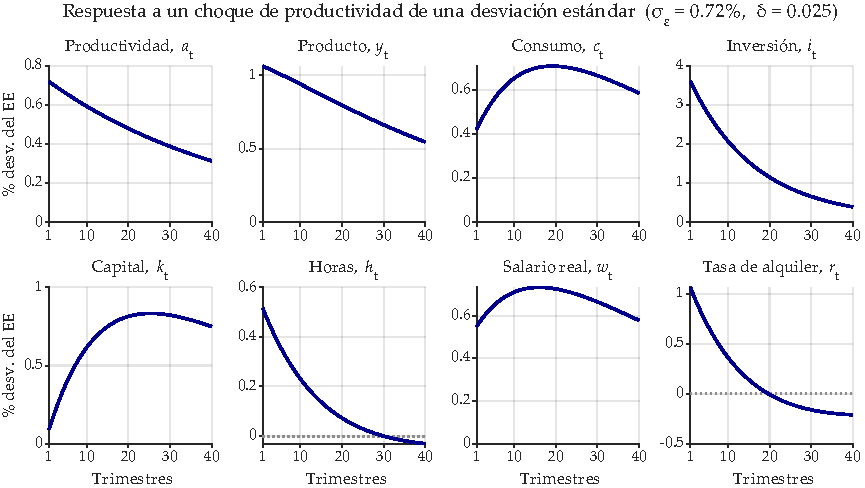
\includegraphics[width=\textwidth]{irf_matlab_base.pdf}
  \par\vspace{0.2cm}\raggedright\small
  Orden sugerido de lectura: $\hat a\to\hat y\to\hat h\to\hat c,\hat\imath\to\hat k\to
  \hat w,\hat r$.
  \fuente{\texttt{oo\_.irfs} de Dynare 7.1, graficadas con \texttt{graficar\_irfs.m}.}
\end{frame}

% S47
\begin{frame}[fragile,label=delta1]{Contraste: depreciación total, $\delta=1$}
  \begin{lstlisting}[language={}]
>> dynare rbc_taller -DDELTA1=1
\end{lstlisting}
  \vspace{0.1cm}
  \centering\small
  \begin{tabular}{@{}lrr@{}}
    \toprule
    \textbf{Impacto, $t=1$ (\%)} & $\delta=0.025$ & $\delta=1$\\
    \midrule
    Producto & 1.064 & 0.720\\
    Consumo & 0.420 & 0.720\\
    Inversión & 3.611 & 0.720\\
    Horas & 0.515 & \num{0}\\
    Persistencia del capital & 0.936 & 0.333\\
    \bottomrule
  \end{tabular}
  \par\vspace{0.3cm}\raggedright\normalsize
  No sobrevive capital: la riqueza es solo el producto de hoy. El hogar consume
  siempre la misma fracción, $c/y=1-\beta(1-\alpha)=0.672$.\par
  \vspace{0.15cm}
  Sin suavizamiento, sustitución e ingreso se cancelan exactamente.
  \fuente{Caso de \textcite{longplosser1983}.}
  \note{Recalibra theta a 3.968. Dynare no guarda oo\_.irfs.h\_eps: la IRF es nula.}
\end{frame}

% S48
\begin{frame}[label=delta1-fig]{Con $\delta=1$, las horas quedan planas}
  \centering
  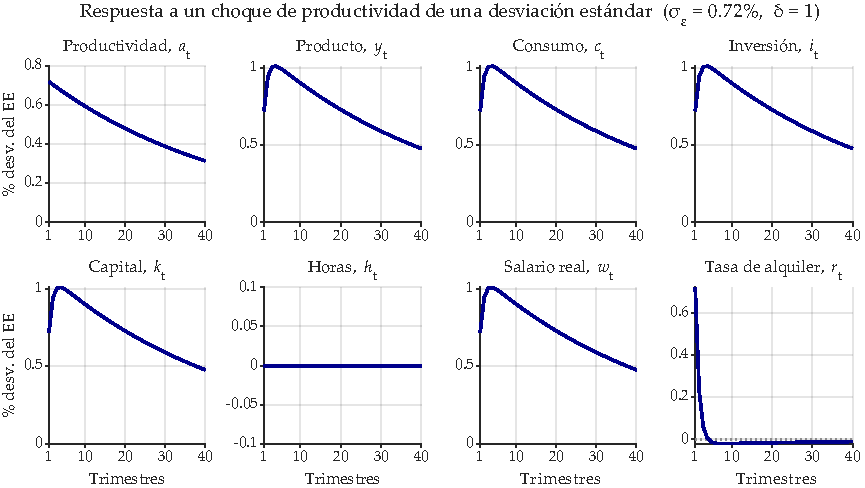
\includegraphics[width=\textwidth]{irf_matlab_delta1.pdf}
  \par\vspace{0.2cm}\raggedright\small
  Producto, consumo, inversión, capital y salario responden \emph{igual} en
  porcentaje: todos son $\hat y_t$, un AR(2) con raíces $\phi$ y $1-\alpha$.
\end{frame}

% S49
\begin{frame}[label=clave]{La ecuación que resume todo}
  Oferta y demanda de trabajo combinadas:
  \[
  \hat y_t-\hat c_t=\frac{\hat h_t}{1-h_{ss}}=1.25\,\hat h_t
  \]
  \begin{center}\large\textbf{Las horas se mueven si y solo si se mueve $c/y$}\end{center}
  \vspace{0.2cm}
  \begin{columns}[T,onlytextwidth]
    \begin{column}{0.48\textwidth}
      \textbf{$\delta=0.025$, $t=1$}\par
      \vspace{0.1cm}
      $1.064-0.420=0.644=1.25\times0.515$\par
      \vspace{0.1cm}
      $c/y$ cae porque el hogar suaviza: las horas suben.
    \end{column}
    \begin{column}{0.48\textwidth}
      \textbf{$\delta=1$, todo $t$}\par
      \vspace{0.1cm}
      $0.720-0.720=0\ \Rightarrow\ \hat h=0$\par
      \vspace{0.1cm}
      $c/y$ es fijo: no hay capital con qué suavizar.
    \end{column}
  \end{columns}
  \par\vspace{0.35cm}
  El capital no solo propaga el choque: es lo que \textbf{activa} la sustitución
  intertemporal del trabajo.
\end{frame}

% S50
\begin{frame}[label=graficos]{De la salida de Dynare a una figura legible}
  \begin{columns}[T,onlytextwidth]
    \begin{column}{0.48\textwidth}
      \centering\textbf{Antes}\par\vspace{0.15cm}
      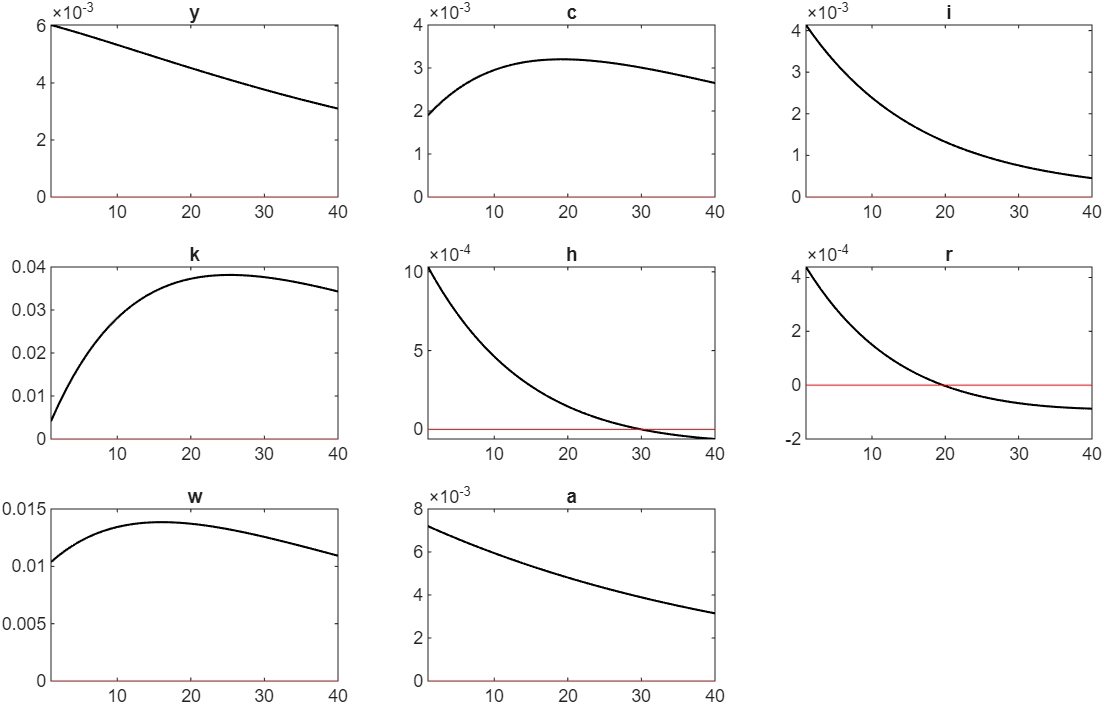
\includegraphics[width=\linewidth]{irf_dynare_default.png}
    \end{column}
    \begin{column}{0.48\textwidth}
      \centering\textbf{Después}\par\vspace{0.15cm}
      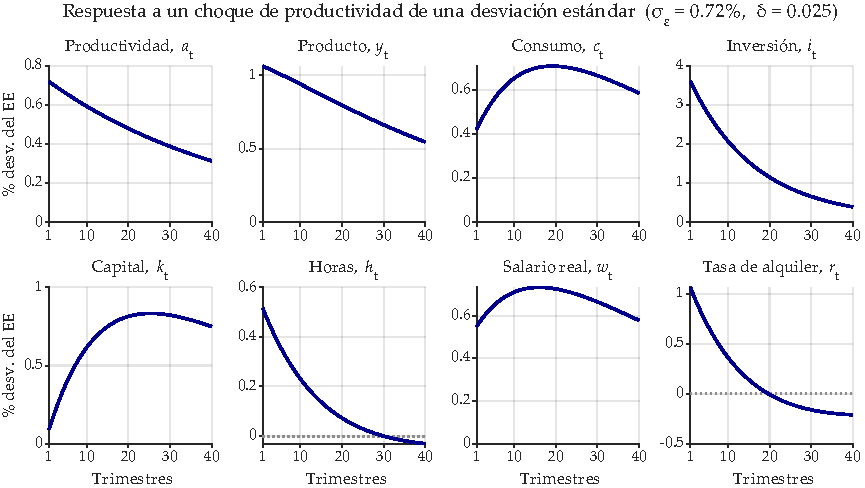
\includegraphics[width=\linewidth]{irf_matlab_base.pdf}
    \end{column}
  \end{columns}
  \par\vspace{0.35cm}\small
  \texttt{graficar\_irfs.m}: una unidad común (\% del EE), títulos con nombre y símbolo,
  ejes que incluyen el cero y tamaño final para imprimir.
  \fuente{Handout, §3.8.3.}
\end{frame}

% ============================================================================
%  5. DATOS Y CIERRE  (165--180 min)
% ============================================================================
\section{Cierre}

% S51
\begin{frame}[label=vs-datos]{El modelo frente a los datos}
  \centering\small
  \renewcommand{\arraystretch}{1.25}
  \begin{tabular}{@{}lcccc@{}}
    \toprule
    & \multicolumn{2}{c}{\textbf{Vol.\ relativa a $y$}} & \multicolumn{2}{c}{\textbf{Corr.\ con $y$}}\\
    \cmidrule(lr){2-3}\cmidrule(lr){4-5}
    & Modelo & Datos & Modelo & Datos\\
    \midrule
    Consumo & 0.44 & 0.53 & 0.94 & 0.82\\
    Inversión & 3.38 & 3.91 & 0.99 & 0.93\\
    Horas & \num{0.49} & \num{1.23} & 0.97 & 0.87\\
    Salario & 0.54 & 0.63 & \num{0.98} & \num{0.22}\\
    \bottomrule
  \end{tabular}
  \par\vspace{0.3cm}\raggedright\normalsize
  Componente cíclico, filtro HP con $\lambda=1600$: en Dynare basta añadir
  \texttt{hp\_filter = 1600} a \texttt{stoch\_simul}.\par
  \vspace{0.2cm}
  Acierta el orden de volatilidades: la inversión es mucho más volátil que el producto
  y el consumo, más suave.
  \fuente{Filtro de \textcite{hp1997}. Datos: EE.UU.\ 1954--2015, \textcite[Tabla~1.2]{gmo}. Modelo: momentos teóricos
  de Dynare. Handout, Cuadro~3.15.}
  \note{$\sigma_y$ del modelo filtrado: 1.4\%, frente a 1.5\% en los datos.}
\end{frame}

% S52
\begin{frame}[label=limites]{Dos cosas que este RBC no logra explicar}
  \begin{columns}[T,onlytextwidth]
    \begin{column}{0.48\textwidth}
      \textbf{1. Poca propagación propia}\par
      \vspace{0.2cm}
      $\hat y/\hat a$: $1.48$ en $t=1$; $1.74$ en $t=40$.\par
      \vspace{0.2cm}
      La forma de $\hat y$ copia la de $\hat a$: casi toda la persistencia viene de
      $\phi=0.979$, no del modelo.
      \fuente{\textcite{cogleynason1995}.}
    \end{column}
    \begin{column}{0.48\textwidth}
      \textbf{2. Horas poco volátiles}\par
      \vspace{0.2cm}
      Modelo: $0.49$ veces el producto. Datos: $1.23$.\par
      \vspace{0.2cm}
      Aun con sustitución intertemporal, las horas se mueven poco. Motiva el trabajo
      indivisible y otras extensiones.
      \fuente{\textcite{hansen1985}.}
    \end{column}
  \end{columns}
  \par\vspace{0.5cm}
  ¿Y el salario? En el modelo es la productividad laboral, $w=\alpha y/h$: con un solo
  choque, todo se mueve al unísono.
  \note{Vuelve la pregunta de la slide impulso: la persistencia viene del choque, no de la
  propagación.}
\end{frame}

% S53
\begin{frame}[label=resumen]{La historia en una tabla}
  \centering\scriptsize
  \renewcommand{\arraystretch}{1.3}
  \setlength{\tabcolsep}{4pt}
  \begin{tabular}{@{}llll@{}}
    \toprule
    \textbf{Momento} & \textbf{Ecuación} & \textbf{Número} & \textbf{Mecanismo}\\
    \midrule
    Impacto: horas & $\hat h=1.715(\hat a-\hat c)$ & 0.515 & sustitución\\
    Impacto: producto & $\hat y=\hat a+\alpha\hat h$ & 1.064 & amplificación\\
    Impacto: reparto & $\hat y=0.798\hat c+0.202\hat\imath$ & 69\% invertido & suavizamiento\\
    Capital & $\Delta\hat k=\delta(\hat\imath-\hat k)$ & máx.\ en $t=26$ & acumulación lenta\\
    Consumo & $\Delta\hat c=\beta r_{ss}\hat r$ & máx.\ en $t=19$ & Euler\\
    Regreso & $\hat h<0$ desde $t=30$ & $-0.031$ en $t=40$ & efecto riqueza\\
    Contraste $\delta=1$ & $\hat y-\hat c=1.25\hat h$ & $\hat h=0$ & $c/y$ constante\\
    \bottomrule
  \end{tabular}
  \par\vspace{0.35cm}\raggedright\normalsize
  Todos los números: la receta o \texttt{oo\_.irfs} en Dynare.
\end{frame}

% S54
\begin{frame}[fragile,label=estimacion]{Siguiente paso: estimar en vez de calibrar}
  Hoy fijamos los parámetros. Dynare también puede \textbf{estimarlos} con datos:\par
  \vspace{0.25cm}
  \begin{enumerate}
    \item La solución se escribe en forma estado-espacio.\par\vspace{0.1cm}
    \item El filtro de Kalman da la verosimilitud de los datos.\par\vspace{0.1cm}
    \item Bayes: posterior $\propto$ verosimilitud $\times$ prior.\par\vspace{0.1cm}
    \item MCMC recorre la posterior.
  \end{enumerate}
  \vspace{0.2cm}
  \begin{lstlisting}
varobs y;
estimated_params; phi, beta_pdf, 0.9, 0.05; end;
estimation(datafile = datos, mh_replic = 20000);
\end{lstlisting}
  \fuente{Esquema ilustrativo. Handout, §3.14.}
  \note{Solo un adelanto: no correr en clase. La sintaxis completa y sus supuestos están en
  el handout.}
\end{frame}

% S55
\begin{frame}[label=material]{Para seguir practicando}
  \textbf{En el repositorio}\par
  \vspace{0.15cm}
  \small
  \begin{tabular}{@{}ll@{}}
    \texttt{handout/handout\_dynare.tex} & el handout completo\\
    \texttt{handout/rbc\_analytical.mod} & el modelo de referencia\\
    \texttt{handout/graficar\_irfs.m} & IRF con estilo\\
    \texttt{handout/reconstruir\_irf.m} & IRF a mano desde \texttt{oo\_.dr}\\
    \texttt{handout/cuatro\_formas/} & el mismo modelo, cuatro escrituras\\
    \texttt{taller/rbc\_taller.mod} & el taller de hoy
  \end{tabular}
  \par\vspace{0.4cm}\normalsize
  \textbf{Ejercicios del handout}\par
  \vspace{0.15cm}
  Barrido en $\phi$, segundo orden, filtro HP, romper el timing y las cuatro formas con
  $\delta=1$.
\end{frame}

% S56
\begin{frame}[label=referencias]{Referencias: método y herramientas}
  \renewcommand*{\bibfont}{\footnotesize}
  \printbibliography[heading=none,keyword=metodo]
\end{frame}

% S57
\begin{frame}[label=referencias-modelo]{Referencias: el modelo}
  \renewcommand*{\bibfont}{\footnotesize}
  \printbibliography[heading=none,keyword=modelo]
\end{frame}

